\documentclass{book}

\usepackage{fullpage}
\usepackage{graphicx}
\usepackage[absolute]{textpos}
\usepackage{parskip}
\usepackage{hyperref}

\begin{document}

\title{CIS 451 Database Processing - Final Project}
\author{Nikki DelRosso}
\date{March 21, 2012}
\maketitle
\thispagestyle{empty}
\let\cleardoublepage\clearpage

\tableofcontents
\newpage

\section{Summary}

This project is a recreation of an old user community website named Shukumei Beta.  The website is a fairly standard user-based website with forums and private messaging, with the inclusion of animal-based characters which users can use for the base of their own stories and forum roleplay characters.  Most of the data being stored is textual user content, such as profiles, forum posts, character descriptions, and messages.  Other applications than those previously mentioned should be administrator and moderator features to maintain the website and moderate the community.

A live version of the project can be viewed at \url{http://nikkidelrosso.com/projects/cis451-final/}.

The database for this assignment can be accessed at ix.cs.uoregon.edu:3297 with the username and password {\bf guest}.

\section{Logical Design}

The following relationships exist in the system:

\begin{itemize}
	\item {\bf User}s may have one {\bf user profile}.
	{\bf User}s may have many
	{\bf roles},
	{\bf alerts},
	{\bf news posts},
	{\bf forum posts},
	{\bf forum threads},
	{\bf game scores},
	{\bf conversation messages},
	{\bf characters},
	{\bf signatures} and
	{\bf friends}.
		
	\item Each {\bf alert} belongs to one {\bf user}.
		
	\item Each {\bf role} may have many {\bf user}s assigned to it.

	\item Each {\bf news entry} may have one {\bf user} as its author.

	\item Each {\bf item} may have one {\bf user} as its owner, and one {\bf item definition}.  Each {\bf item definition} may be in several {\bf item type categories}.  Each {\bf item type category} may have several {\bf item definition}s associated with them.

	\item Each {\bf character} has one {\bf species}, one {\bf color}, and one owner.  Many {\bf character}s may share the same {\bf species} and/or {\bf color}.  There is one {\bf image} for each {\bf species}/{\bf color} combination.

	\item A {\bf game} may have been {\bf score}d on many times.  Each {\bf game score} is made by a single {\bf user}.

	\item A {\bf forum post} has one {\bf user} as an author, and one {\bf thread}.  A thread has many posts, and one {\bf forum}.  A {\bf forum} has many {\bf thread}s, and one {\bf category}.  A category has many {\bf forum}s.
\end{itemize}

A relational diagram of the above relations can be seen on the next page.

\newpage
\hspace{\textwidth}\\
\begin{textblock}{0}(2.5,1) 
	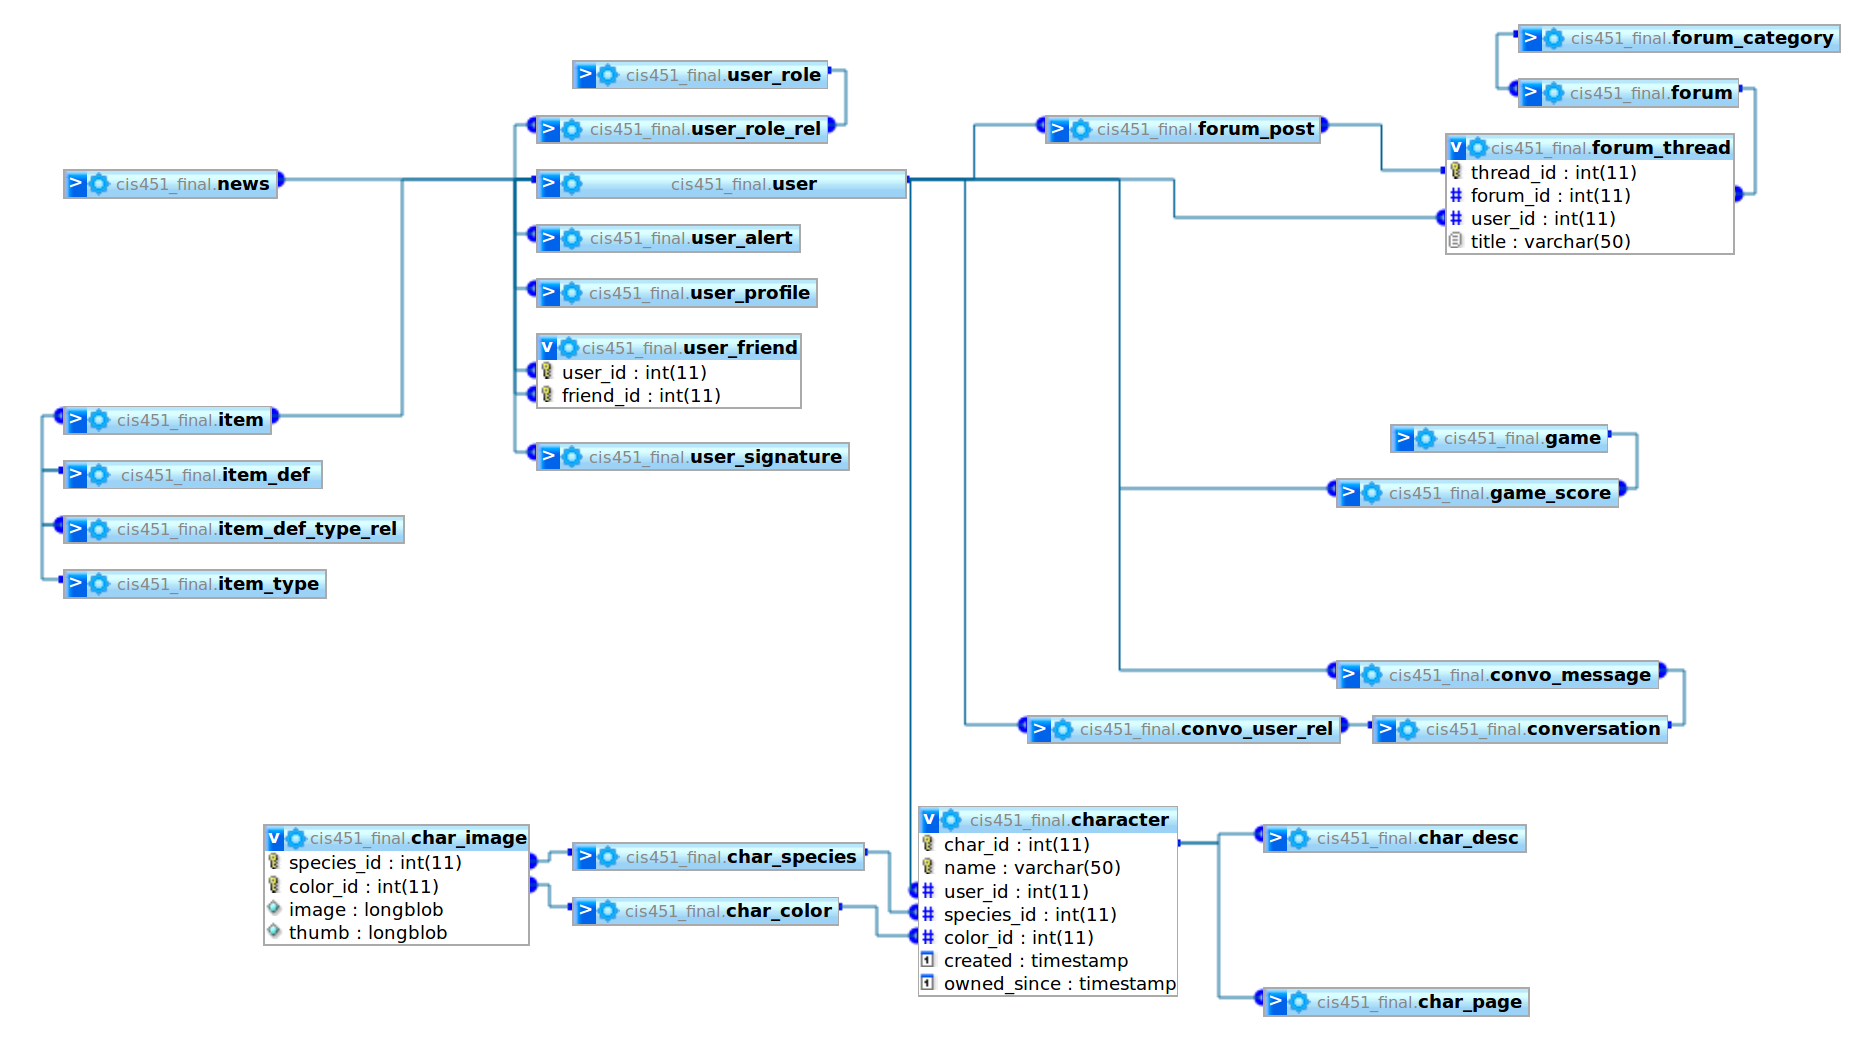
\includegraphics[angle=90,width=5in]{diagram.png}
\end{textblock}
\newpage

\section{Physical database design}
Normalization of the data is mostly natural based on the relationships between them.  Columns which may take a large amount of space are stored in different tables (such as user profiles, and character descriptions) to avoid selecting unecessary amounts of data; since these columns are also frequently empty, this prevents columns from reserving an excess amount of data and fewer nulls in the user and character tables.  Another benefit to storing these things in separate tables is the ease of transition from a one-to-one relationship to a one-to-many relationship, which I had expressed as a potentially desirable feature in the future for character pages.

Another design decision is to use numeric, auto-increment IDs to relate tables to one another, as opposed to using unique varchar columns (e.g. usernames).  This both reduces the space to store foreign keys, and makes the ability to change names very easy.

A dump including the definition for each table has been attached with the submission of this final, and can also be found at \\ \url{http://nikkidelrosso.com/projects/cis451-final/data/database.sql}

\section{Physical application design}
These are the descriptions for the implemented applications.
\subsection{Forums}
Users can post threads and posts replying to threads on boards categorized by forums and forum categories.  This reads the user, forum category and forum tables while writing the forum thread and forum post tables.

\subsection{User profiles}
A list of all users can be viewed (reads the user table).  A profile page for each individual user can be viewed, displaying that user's profile content, data such as date joined and number of posts on the forums, and that users characters (reads the user, character, user profile, and forum post tables).  User profiles can also be edited (writes the user profile table).

\subsection{Character descriptions}
Characters each have their own pages containing some basic information, an image of the character, and a profile editable by administrators and that character's owner.  The profile display reads the character and character description tables, while the edit modifies the description table.


\newpage
\section{User's guide}
There is no login implemented for this site; instead, a hard-coded "guest" account has been added.

To access the forums, click on the "forum" link at the top of the page.  From here, select the desired forum to view.  A new thread can be posted in this forum using the form at the bottom of the thread list, or a thread title can be clicked on to view the posts in that thread.  When viewing a thread, again there is a form at the bottom of the page to post a reply.

To access your user profile (for the guest account), click on either "accounts" at the top of the page, or in the user informational bar below the header, click on your username.  You can then edit your profile by clicking the "edit profile" link at the top of the content on this page.

Character profiles can be viewed by clicking on the character on a user profile.  Character profile contents can also be edited in the same way as user profiles.

404 pages will be encountered when trying to browse unimplemented features on the site.

\section{Table contents}
The structure and contents of the database can be found in a dump at \\ \url{http://nikkidelrosso.com/projects/cis451-final/data/database.sql}

\section{Implementation code}
This application was custom built with the exception of the Savant3 PHP templating library as sort of a "query-view-controller" system.  An .htaccess file routes all requests through an index.php file in the root of the project.  Static files are the one exception to this routing, and are served from the static/ directory.  From here, the index.php file tries to find a handler for the application specified by the URL; first it checks to see if it has a rule fo the given URL, and if not it looks for a handler.php file in the first subdirectory of the URL (ex: the request for "/forum/announcements/1/" would either route to the rule defined for "forum", or try to use a "forum/handler.php").  The handlers then tend to manage the rest of the URL using regular expressions; each different aspect of each application tends to have its own file to fetch data from the database, and a template to display that information.

The implementation code can be found here: \url{http://github.com/nikker/cis451/}

\newpage
\section{Conclusion}
Implemented applications:
\begin{itemize}
	\item Forums: Viewing list of forums by category, viewing lists of threads in forums and lists of posts in threads, posting replies to threads, and posting new threads.
	\item User list: List of all users in the database with a link to their profile.
	\item User profiles: User profile information including data about the user and an editable section, and a list of that users characters.
	\item Character descriptions:  Character profiles with an editalble description.
\end{itemize}

There are a lot of things that I would have liked to include in this project, but could not complete in the time constraints.  Many of these are site features, such as: a character creation form, private messaging system, user items and inventory, et cetera.  To use this code outside of a class assignment, I would also like to turn it into a true model-view-controller by creating actual database models instead of just using pure SQL.


\end{document} 
